%Preambuła
\documentclass[a4paper,10pt]{article}
\usepackage[polish]{babel}
\usepackage[OT4]{fontenc}
\usepackage[utf8]{inputenc}
\usepackage{array}
\usepackage{subfloat}
\usepackage[T1]{fontenc}
\usepackage{caption}
\usepackage{float}
\usepackage{verbatimbox}
\usepackage{numprint}
\usepackage{hyperref}
\usepackage{graphicx}
%\usepackage[export]{adjustbox}

\DeclareGraphicsExtensions{.pdf,.png,.jpg}

\newcolumntype{R}[1]{>{\raggedleft\arraybackslash}p{#1}}
\newcolumntype{C}[1]{>{\centering\arraybackslash}p{#1}} 
\newcolumntype{L}[1]{>{\raggedright\arraybackslash}p{#1}}

% Część główna

\title{Techniki Analizy Sieci Społecznych (TASS)\\Projekt 1: Analiza statystyczna grafu przy użyciu standardowych narzędzi}
\author{Andrzej Smyk}
\date{9 kwietnia 2015}
\begin{document}
	\maketitle
	
	\section{Cel projektu}
	Celem projektu jest zapoznanie się z podstawowymi narzędziami służącymi do analizy sieci społecznych. Wszystkie zadania projektowe powinny zostać zrealizowane przy wykorzystaniu funkcji z pakietu \textit{NetworkX} języka \textit{Python 2.7.6} oraz za pomocą programu \textit{Pajek 4.02}.

	Pierwszym zadaniem jest estymacja współczynnika rozkładu stopni wierzchołków. Kolejne zadania dotyczą wyznaczenia 10 wierzchołków o największym pośrednictwie (\textit{betweenness}) oraz obliczenia długości najdłuższej spójnej składowej. Wymienione eksperymenty zostaną również przeprowadzone dla grafu z usuniętą połową wierzchołków.

	\section{Opis danych}
	Dane do projektu pochodzą ze strony: \linebreak\url{https://sites.google.com/site/bctnet/datasets}. Dotyczą one funkcyjnej współpracy różnych obszarów całego ludzkiego mózgu. Plik zawiera macierz sąsiedztwa oraz macierz współrzędnych. W sumie graf składa się z 638 wierzchołków oraz z 18625 krawędzi. 

	Dane zapisane były w formacie MATLAB'a \texttt{mat}, więc na początek załadowałem go do Pythona za pomocą funkcji \texttt{loadmat()} z modułu \texttt{scipy.io}. Następnie, wczytane macierze wykorzystałem do stworzenia nieskierowanego grafu za pomocą funkcji pakietu NetworkX. By sprawdzić czy graf jest rzeczywiście nieskierowany, porównałem kolejne elementy z transponowanej macierzy sąsiedztwa z nią samą. Dzięki temu upewniłem się, że poprawnie wczytałem graf.

	Ponieważ Pajek nie ma wsparcia dla formatu \texttt{mat}, wykorzystałem funkcję \texttt{write\_pajek()} do zapisania wygenerowanego grafu w formacie \texttt{net}. Wcześniej, dodałem jeszcze etykiety z numeracją węzłów. Podobnie postąpiłem z grafem, z którego usunąłem połowę wierzchołków. Losowy wybór wierzchołków do usunięcia zagwarantowałem korzystając z funkcji \texttt{sample} z modułu \texttt{random}. Za jej pomocą wygenerowałem próbkę wierzchołków o wielkości równej połowie grafu, a następnie usunąłem wylosowane wierzchołki.

	Wszystkie wygenerowane pliki dołączyłem do sprawozdania. Plik \linebreak\texttt{Coactivation\_matrix.mat} zawiera oryginalne macierze. Pliki \mbox{\texttt{coa\_matrix.net}} i \mbox{\texttt{coa\_matrix\_half.net}} zostały wygenerowana przy pomocy NetworkX i zawierają grafy odpowiednio ze wszystkimi oraz z połową wierzchołków.

	\section{Estymacja wykładnika charakterystycznego}
		Wszystkie opisane poniżej kroki analizy przeprowadziłem w oparciu o proste skrypty w językach Python oraz R. Odpowiednie pliki zostały dołączone do sprawozdania i są to kolejno:
		\texttt{network\_analysis.py}, \texttt{estimation.py} i \texttt{pajek\_calcs.r}.

		Pierwszym krokiem było wygenerowanie listy stopni wierzchołków dla wszystkich wierzchołków znajdujących się w grafie. W NetworkX wykorzystałem do tego funkcję \texttt{degree()}. W Pajeku użyłem opcji \textit{Network \textgreater Create Partition \textgreater Degree \textgreater All}. Ponieważ Pajek nie udostępnia wielu opcji operacji nad danymi, listę stopni wierzchołków wyeksportowałem do programu R Studio, gdzie przeprowadziałem dalsze etapy analizy.

		W NetworkX funkcja \texttt{degree()} zwraca słownik z parami ''wierzchołek : stopień''. Korzystając z funkcji \texttt{hist()} z modułu \texttt{matplotlib.pyplot} wyznaczyłem częstości dla 100 przedziałów i wygenerowałem histogram. Alternatywą jest przeanalizowanie wykresu w skali logarytmicznej. Poniżej przedstawiono odpowiednio wykresy: histogram, wykres częstości loglog stopni wierzchołków oraz wykres częstości stopni wierzchołków w zwykłej skali:
		\begin{figure}[H]
			\raggedleft
			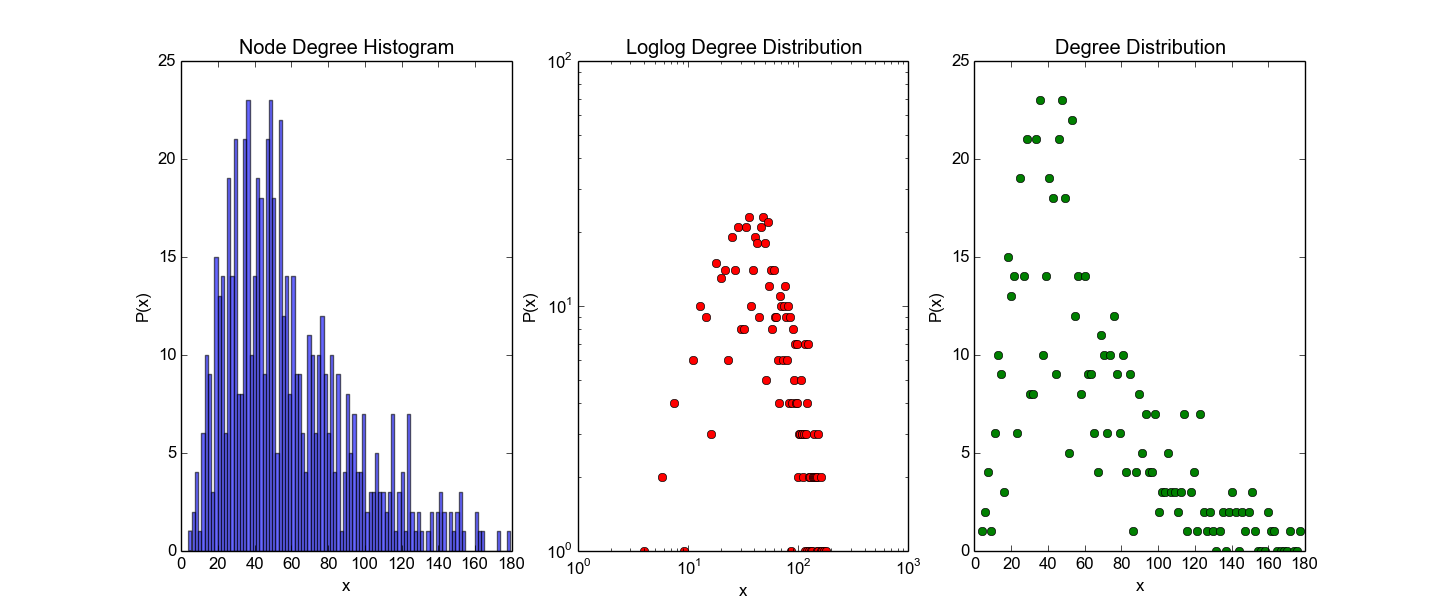
\includegraphics[width=\linewidth, trim=50pt 30pt 50pt 25pt, clip]{figure_1}
			\hfill
		\end{figure}

		Dodatkowo, wygenerowałem adekwatne wykresy, tym razem korzystając z przedziałów logarytmicznych dla histogramu i wyznaczenia przedziałów częstości:
		\begin{figure}[H]
			\raggedleft
			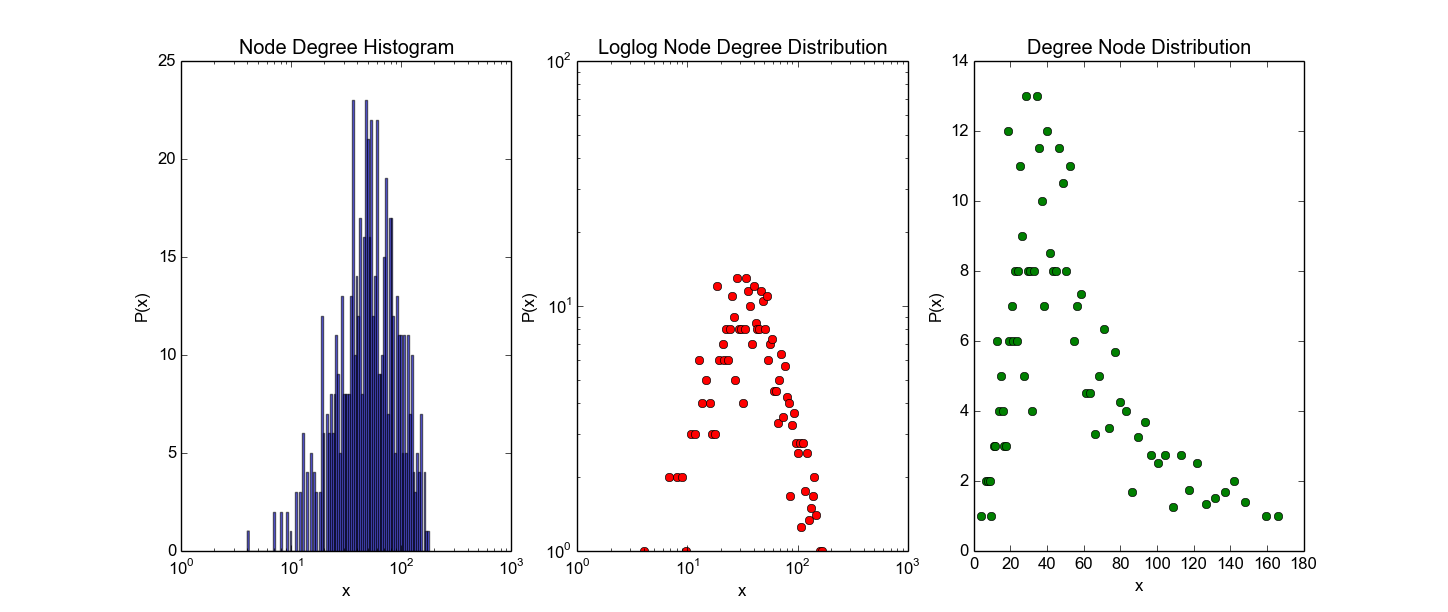
\includegraphics[width=\linewidth, trim=50pt 30pt 50pt 25pt, clip]{figure_2}
			\hfill
		\end{figure}
		Wszystkie wykresy różnią się znacząco od tego, jak powinien prezentować się wykres dla rozkładu potęgowego. Na wykresie loglog powinniśmy widzieć malejącą prostą. Tutaj zaś mamy do czynienia z czymś co przypomina rozkład normalny z grubym ogonem (asymetryczny). Może to sugerować, że w rzeczywistosci mamy do czynienia nie z rozkładem potęgowym, ale podobnym rozkładem log-normalnym.

		Mimo wszystko, spróbuję wyestymować współczynnik rozkładu potęgowego $\hat{\alpha}$. W tym celu napisałem w języku Python prostą funkcję:\\\linebreak
		\begin{verbbox}
			def estimate_alpha(xs, x_min):
	    		from numpy import log, sum
	    		xs_cutoff = [x / (x_min - 0.5) for x in xs if x >= x_min]
	    		return 1 + len(xs_cutoff) / sum(log(xs_cutoff))
		\end{verbbox}
		\fbox{\theverbbox}
		\\\hfill
		Wcześniej, należy jednak wyznaczyć empirycznie wartość $x_{min}$, za którą będziemy wyznaczać estymować parametr rozkładu. Zazwyczaj stosuje się do tego estymator oparty na statystyce Kołomorogowa - Smirnowa. Prostszą, ale bardziej podatną na błędy metodą jest wyestymowanie $\hat{\alpha}$ dla różnych $x_{min}$ i naniesienie takiej zależności na wykres. Można spróbować wskazać odpowiednią wartość, wyszukując punkt poza którym funkcja traci swoją stabilność. Wykres, który w tym celu wygenerowałem jest przedstawiony poniżej:\\\linebreak
		\begin{figure}[H]
			\centering
			\hfill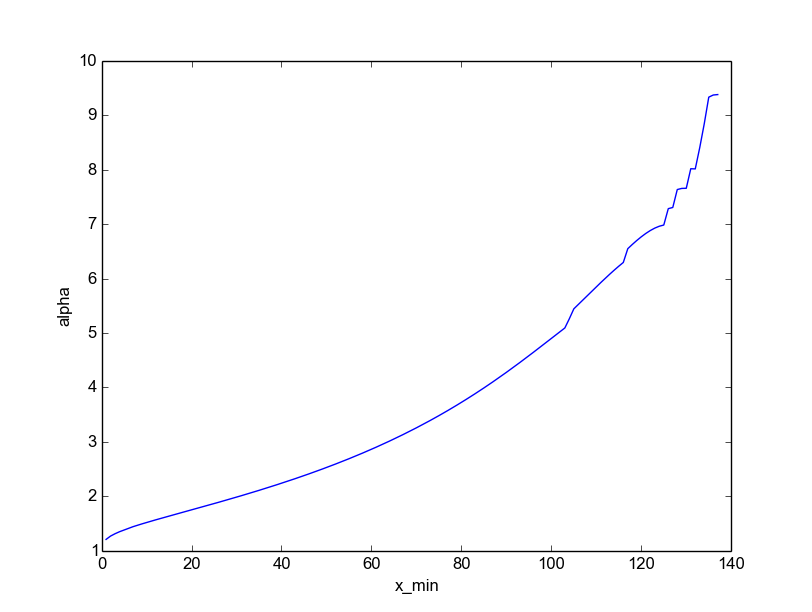
\includegraphics[width=\linewidth]{figure_3}
		\end{figure}

		Wygląda na to, że funkcja przestaje być stabilna na poziomie ok. 103 - 104 wierzchołków. Dla $x_{min} = 104$ wartość $\hat{\alpha} = 5.261$. Dla porównania, obie wartości wyznaczyłem korzystając z funkcji \texttt{Fit()} modułu \texttt{powerlaw}. Uzyskałem w niej podobny wynik $x_{min} = 105$ wartość $\hat{\alpha} = 5.539$. Oczywiście, funkcje zaimplementowane w tym module korzystają z bardziej dokładnych metod, w tym wspomnianej statystyki KS.

		Trochę inne wyniki uzyskałem w wykonując obliczenia w środowisku R Studio, korzystając z pakietu \texttt{poweRlaw}. Funkcje tego pakietu wykorzystują bootstrapping do estymacji
		$x_{min}$ oraz $\hat{\alpha}$. Wartości, które uzyskałem to odpowiednio $x_{min} = 114$ wartość $\hat{\alpha} =6.64$. Różnica względem obliczeń przeprowadzony w Pythonie, może wynikać innej metody estymacji, tj. wykorzystaniu bootstrappingu.

		Dodatkowo przy wykorzystaniu funkcji \texttt{bootstrap\_p()} przeprowadziłem test, w którym za przyjąłem poniższy zestaw hipotez:
		\begin{quote}
		$H_0$: zmienna losowa ma rozkład potegowy\\
		$H_1$: zmienna losowa ma inny rozkład niż potęgowy
		\end{quote}
		Wartość $\textit{p-value} = 0.09$ dla poziomu istotności równego 0.10 pozwala na odrzucenie hipotezy zerowej na rzecz hipotezy alternatywnej. Chociaż wynik ten jest ''na granicy'', można jednak przypuścić, że rozkład stopni wierzchołków grafu nie jest do końca rozkładem potęgowym.\linebreak\\\\

		\pagebreak
	\section{Pośrednictwo - \emph{Betweeness Centrality}}
			W pakiecie NetworkX do wyznaczenia pośrednictwa wierzchołków wykorzystałem funkcję \texttt{betweenness\_centrality(G, normalized=True)}. Następnie uzyskany w ten sposób słownik zamienłem na posortowaną listę i wypisałem za pomocą \texttt{PrettyTables}. 

			W programie Pajek na początku wyznaczyłem wektor zawierający wartości pośednictwa dla każdego wierzchołka. W tym celu wybrałem w menu programu kolejno: \textit{Network \textgreater Create Vector \textgreater Centrality \textgreater Betweeness}. Ponieważ Pajek nie udostępnia opcji sortowania danych wynikowych z obliczeń (lub ja po prostu takiej funkcji nie znalazłem), wektor z danymi wyeksportowałem do pliku \texttt{csv}, który następnie załadowałem do środowiska \textit{R Studio}, gdzie dokonałem wyznaczenia 10 wierzchołków o największym pośrednictwie. 
			Poniższa tabela przedstawia 10 wierzchołków o największym pośrednictwie wyznaczonych dla grafu ze wszystkimi wierzchołkami (638):
			\begin{table}[H]
			\parbox{.45\linewidth}{
			\caption*{Pośrednictwo w \mbox{NetworkX}}
			\begin{tabular}{ c | c } \hline
				Numer wierzchołka & Pośrednictwo \\ \hline
				330 & 0.009784  \\
				621 & 0.009158 \\
				546 & 0.008546 \\
				339 & 0.008065 \\
				629 & 0.007858 \\
				482 & 0.007780 \\
				230 & 0.007731 \\
				235 & 0.007443 \\
				50 & 0.007427 \\
				416 & 0.007342 \\\hline
			\end{tabular}
			}
			\hfill
			\parbox{.45\linewidth}{
			\caption*{Pośrednictwo w Pajek}
			\begin{tabular}{ c | c } \hline
				Numer wierzchołka & Pośrednictwo \\ \hline
				330 & 0.0097836 \\
				621 & 0.0091577 \\
				546 & 0.0085458 \\
				339 & 0.0080647 \\
				629 & 0.0078578 \\
				482 & 0.0077797 \\
				230 & 0.0077312 \\
				235 & 0.0074427 \\
				50  & 0.0074266 \\
				416  & 0.0073421 \\\hline
			\end{tabular}
			}
			\end{table}
			Po usunięciu połowy losowo wybranych węzłów powtórzyłem obliczenia dla grafu składającego się z 319 wierzchołków:
			\begin{table}[H]
			\parbox{.45\linewidth}{
			\caption*{Pośrednictwo w \mbox{NetworkX}}
			\begin{tabular}{ c | c } \hline
				Numer wierzchołka & Pośrednictwo \\ \hline
				431 & 0.019370 \\
				230 & 0.018752 \\
				451 & 0.017337 \\
				418 & 0.016012 \\
				505 & 0.015427 \\
				11  & 0.015216 \\
				629 & 0.014829 \\
				202 & 0.014119 \\
				623 & 0.014114 \\
				452 & 0.013814 \\\hline
			\end{tabular}
			}
			\hfill
			\parbox{.45\linewidth}{
			\caption*{Pośrednictwo w Pajek}
			\begin{tabular}{ c | c } \hline
				Numer wierzchołka & Pośrednictwo \\ \hline
				431 & 0.019370 \\
  				230 & 0.018752 \\
  				451 & 0.017337 \\ 
				418 & 0.016012 \\
				505 & 0.015427 \\
				11 & 0.015216  \\
				629 & 0.014829 \\
				202 & 0.014119 \\
				623 & 0.014114 \\
				452 & 0.013814 \\\hline
			\end{tabular}
			}
			\end{table}
			\pagebreak
	\section{Wyznaczenie długości najdłuższej spójnej składowej}
	Do wyznaczenia długości największego silnie spójnego komponentu w pakiecie NetworkX wykorzystałem funkcję \texttt{connected\_components(G)}, która zwraca wszystkie komponenty (spójne składowe) grafu. Następnie wyznaczyłem długość każdego z nich i wybrałem najdłuższy. W Pajeku do analogicznej operacji wykorzystałem \textit{Network \textgreater Create Partition \textgreater Components \textgreater Weak}. Pajek po wyznaczeniu wszystkich komponentów, w oknie raportu od razu melduje jaka jest długość najdłuższego komponentu. Wynik dla grafu ze wszystkimi wierzchołkami:\\\\
	\begin{verbbox}
		================================================================
		Weak Components
		================================================================
		 Working...
		 Number of components: 1
		 Size of the largest component: 638 vertices (100.000%).
		 Time spent:  0:00:00
	\end{verbbox}
	\fbox{\theverbbox}
	\\\\
	Wynik dla grafu z połową wierzchołków:\\\\
	\begin{verbbox}
		================================================================
		Weak Components
		================================================================
		 Working...
		 Number of components: 1
		 Size of the largest component: 319 vertices (100.000%).
		 Time spent:  0:00:00
	\end{verbbox}
	\fbox{\theverbbox}
	\\\\
	Oba narzędzia pokazały, że dla podanego grafu długość najdłuższej spójnej składowej wynosi 638. Oznacza to, że najdłuższa ścieżka w tym gafie zawiera jego wszystkie wierzchołki, lub inaczej, istnieje możliwość dotarcia z dowolnego węzła do innego, dowolnego, wierzchołka.
	\pagebreak
	\section{Czasy obliczeń}
		Do pomiaru czasu obliczeń w Pythonie wykorzystałem moduł \texttt{timeit}, do którego przekazałem odpowiednie parametry środowiska:
		\begin{verbatim}
			setup = '''
			from __main__ import longest_comp_len, G
			import networkx as nx
			'''
			timeit.timeit("nx.betweenness_centrality(G, normalized=True)", setup, number=1)
			timeit.timeit("longest_comp_len(G)", setup, number=1)
		\end{verbatim}
		Uzyskane czasu obliczeń przedstawia tabela poniżej:
		\npdecimalsign{.}
		\nprounddigits{5}
		\\\\
		\begin{tabular}{ L{5 cm} | c } 
			Parametr (\emph{rozmiar}) & Python \\\hline
			10 wierzchołków o największym pośrednictwie (\emph{638}) & 23.039811 \\
			10 wierzchołków o największym pośrednictwie (\emph{319}) & 3.777321 \\
			Rozmiar największej składowej spójnej (\emph{638}) & 0.006186 \\
			Rozmiar największej składowej spójnej (\emph{319}) & 0.002010 \\ \hline
		\end{tabular}
		\npnoround
		\\\\\newline
		Ponieważ Pajek przy wszystkich obliczeniach podaje jak długo wykonywały się obliczenia, nie ma było potrzeby stosowania dodatkowych narzędzi do przeprowadzenia pomiarów. Okazuje się, że wszystkie obliczenia zostały wykonane w czasie krótszym niż sekunda. O ile dla wyznaczenia długości najdłuższej spójnej składowej, nie odbiegają one od czasów w NetworkX, to już zdecydowanie szybsze wyznaczenia wielkości pośrednictwa nastąpiło znacznie szybciej. Różnica ta może wynikać z dobrej optymalizacji algorytmów w Pajeku oraz z ograniczeń interpretera Pythona. Raport z programu Pajek znajduje się w pliku \texttt{pajek\_report.rep}.
\end{document}

